\chapter{Implementation and Results}

This chapter aims to provide a high-level algorithm that can be used to implement the solution provided in the previous Chapter. We will also present and discuss the results achieved from the implementation of the proposed method. Before moving forward let us reiterate the problem statement. There exists a gap in research for methods to track objects or people in three-dimensional space that needs no pre-preparation or a lot of special equipment to gather data. the aim of this thesis is to find that requires neither of those two things and can work on a monocular RGB vision image or video, captured by a regular phone camera.\newline

The idea to solve this is to use the vanishing points existing in the space to figure out the depth of the person/object in consideration and continue tracking of the coordinates found using the depth gives the trajectory of the person as they move through the image space. so we first need to figure out where the vanishing points lie in the space, and then we need to find the boundaries of the walls present in the scene then using the method proposed in the previous chapter, we find the coordinates of the subject and do this over and over for each new frame essentially tracking them.\newline

\section{Implementation}

\section{Results}

In this section, we will discuss the experimental setup and the results obtained at each step of the implementation of the method.\newline

\subsection{The Experimental Setup}

For our experimental setup, we have monocular images of different places in different perspective views, we also have monocular video streams In different orientations and perspective views. These images are then processed in Python to obtain the results which are shown in the sections that follow.\newline

\subsection{Mapping the room}

To map the room effectively we essentially need to find the corners and the edges of the walls and then using the Contextual information that can be extracted from the walls and the floor and the roof of the room figure out the perspective view that the image exists in. further we need to figure out the centroid of the vanishing points.\newline

Some metals that can be used to do so are edge detection filters, line detection algorithms, corner detection algorithms, and image segmentation models, for our testing we have used image segmentation along with these other techniques to figure out the weighted vanishing point, or in other words the centroid of the vanishing point.\newline

\begin{figure}[H]
    \centering
    \includegraphics[width=1.0\textwidth]{1vp room.jpg}
    \caption{A room in 1VP perspective view}
    \label{fig: A room in 1VP perspective view}
\end{figure}


\ref{fig: A room in 1VP perspective view} and \ref{fig: A room in 3VP perspective view} represent two rooms in 1VP perspective view and 3VP prespective view respectively. These images are passed through an image segmentation algorithm to detect walls. \ref{fig: 1VP perspective view room segmentation} and \ref{fig: 3VP perspective view room segmentation}  showcase he result obtained from the segmentation algorithm. The boundary marked in green is the segmentation boundary.\newline

\begin{figure}[H]
    \centering
    \includegraphics[width=1.0\textwidth]{1vp Segmentation Result.png}
    \caption{1VP perspective view room segmentation}
    \label{fig: 1VP perspective view room segmentation}
\end{figure}

\begin{figure}[H]
    \centering
    \includegraphics[width=1.0\textwidth]{1vp Segmentation and Corner Detection Result.png}
    \caption{1VP perspective view line detection}
    \label{fig: 1VP perspective view line detection}
\end{figure}

\ref{fig: 1VP perspective view line detection} and \ref{fig: 3VP perspective view line detection} show the lines marked using the segmentation boundaries. As \ref{fig: A room in 1VP perspective view} to \ref{fig: 1VP perspective view Weighted Vanishing Point} represent a rather simple scene it is easy to see that most of the lines marked with the help of the segmentation boundary lead to the centre of the image which also is the only vanishing point. However, for more complex scenes such as the one presented in Figure 5-8 to Figure 5-12, it is not that easy to see the vanishing points.\newline

\begin{figure}[H]
    \centering
    \includegraphics[width=1.0\textwidth]{1vp Most Converged Area.png}
    \caption{1VP perspective view Vanishing point possibility space}
    \label{fig: 1VP perspective view Vanishing point possibility space}
\end{figure}

Figure \ref{fig: 1VP perspective view Vanishing point possibility space} and \ref{fig: 3VP perspective view Vanishing point possibility space} show the area that has points where multiple lines intersect, it is important to note that a lot of these points don’t neceseraly have receding parallel lines intersecting at them, but lines that are orthogonal to the vanishing points. Because these are not special points they are distrtributed over the entire image space and don’t really contribute in finding the weighted vanishing point.\newline

\begin{figure}[H]
    \centering
    \includegraphics[width=1.0\textwidth]{1vp Centroid of Most Converged Area.png}
    \caption{1VP perspective view Weighted Vanishing Point}
    \label{fig: 1VP perspective view Weighted Vanishing Point}
\end{figure}

\ref{fig: 1VP perspective view Weighted Vanishing Point} and \ref{fig: 3VP perspective view Weighted Vanishing Point} Show the weighted vanishing point that can later be used to calculate the ratios and further the depth and coordinates of the people/objects present in the scene.\newline

\begin{figure}[H]
    \centering
    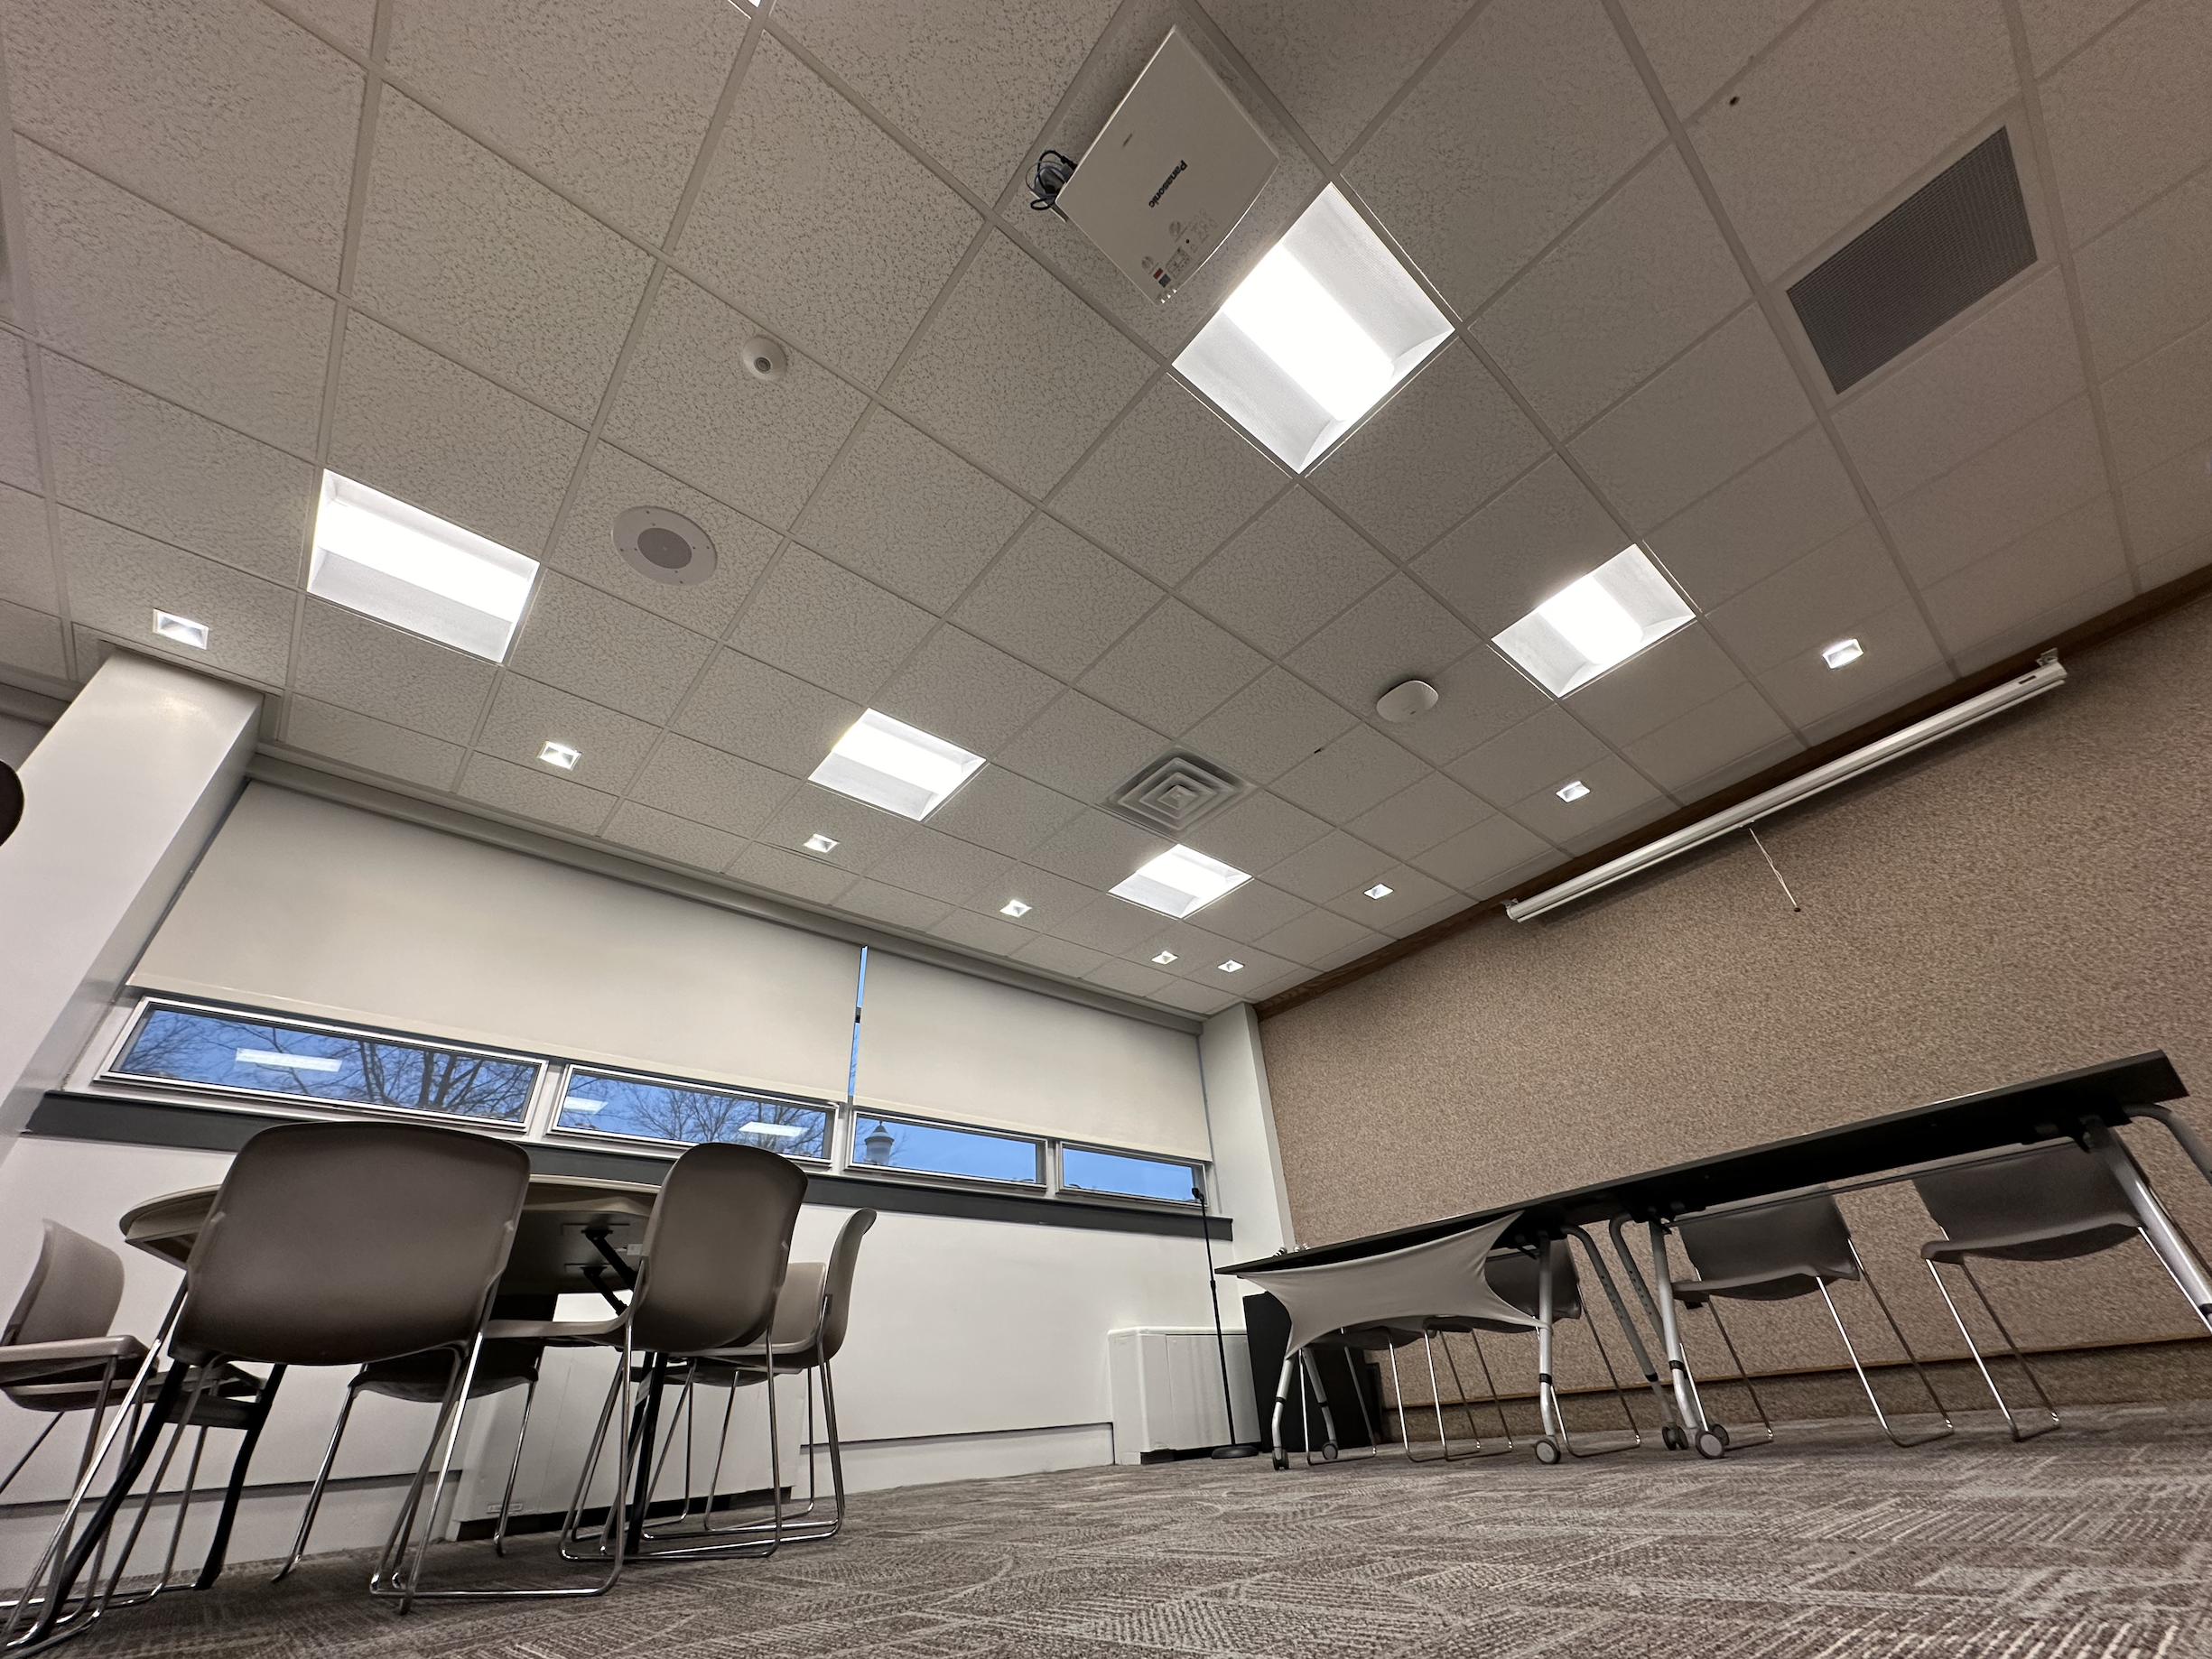
\includegraphics[width=0.8\textwidth]{3vp.png}
    \caption{A room in 3VP perspective view}
    \label{fig: A room in 3VP perspective view}
\end{figure}

\begin{figure}[H]
    \centering
    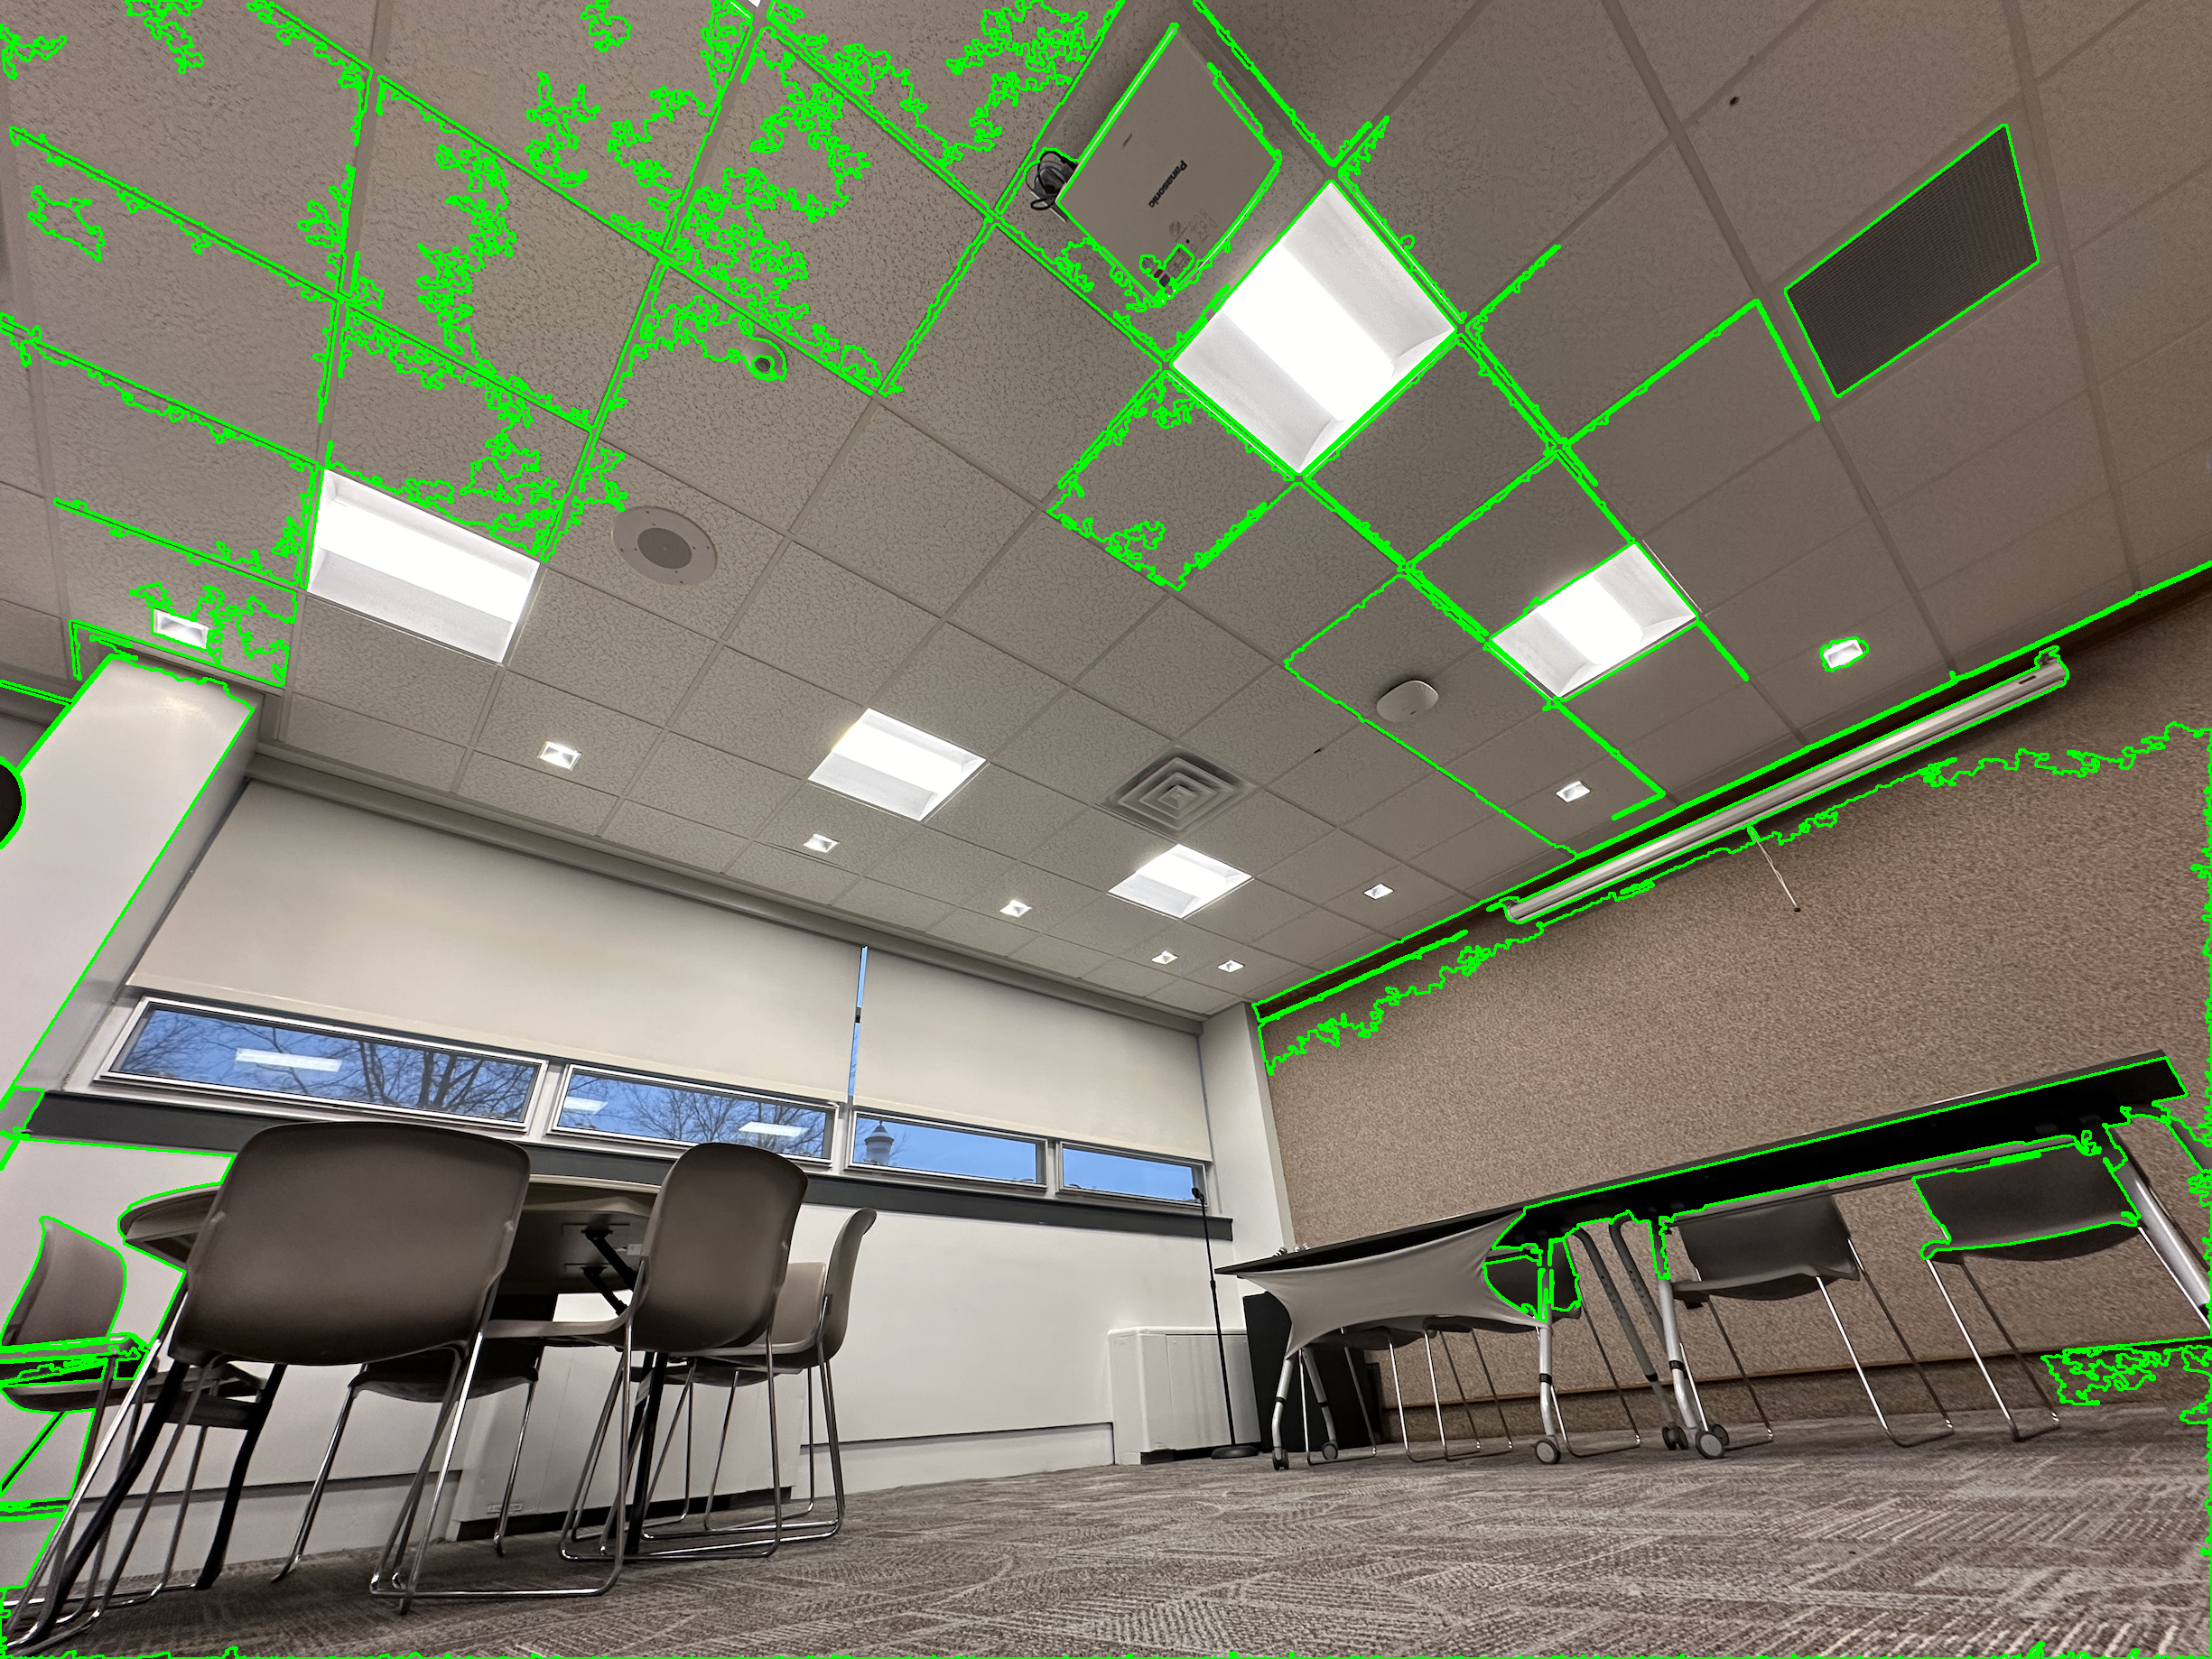
\includegraphics[width=0.8\textwidth]{3vp Segmentation Result.png}
    \caption{3VP perspective view room segmentation}
    \label{fig: 3VP perspective view room segmentation}
\end{figure}

\begin{figure}[H]
    \centering
    \includegraphics[width=0.8\textwidth]{3vp Segmentation and Corner Detection Result.png}
    \caption{3VP perspective view line detection}
    \label{fig: 3VP perspective view line detection}
\end{figure}

\begin{figure}[H]
    \centering
    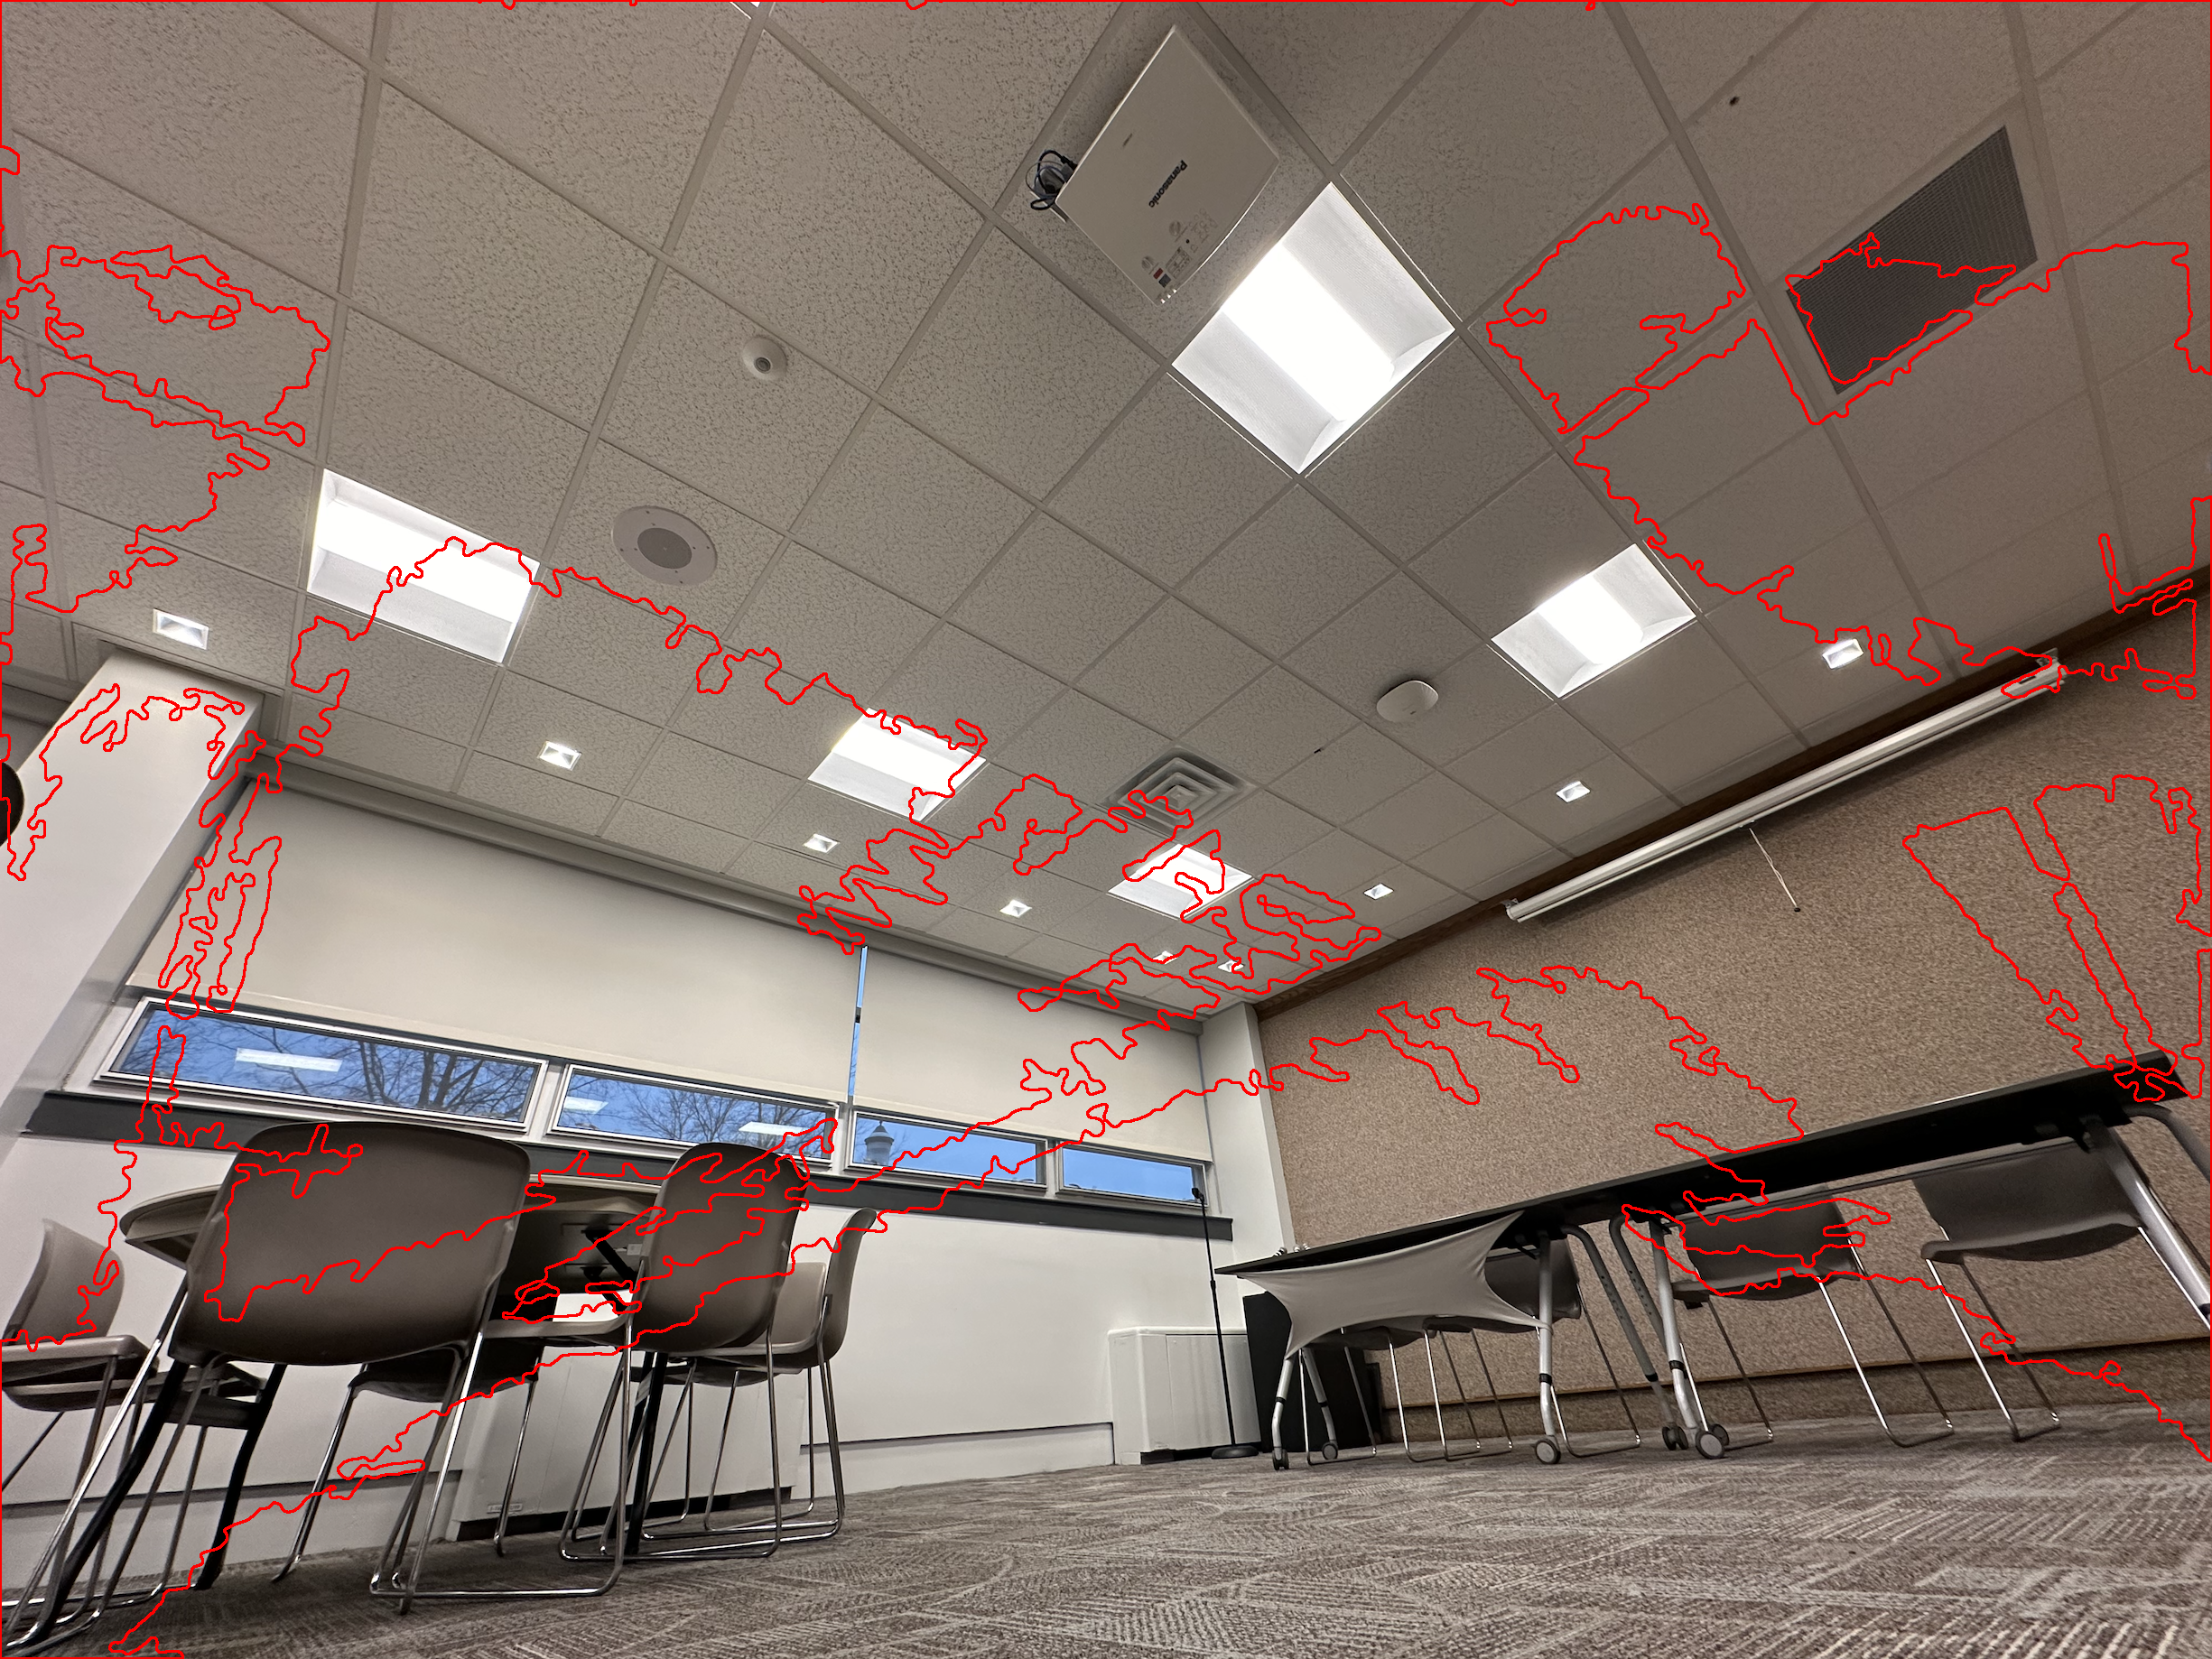
\includegraphics[width=0.8\textwidth]{3vp Most Converged Area.png}
    \caption{3VP perspective view Vanishing point possibility space}
    \label{fig: 3VP perspective view Vanishing point possibility space}
\end{figure}

\begin{figure}[H]
    \centering
    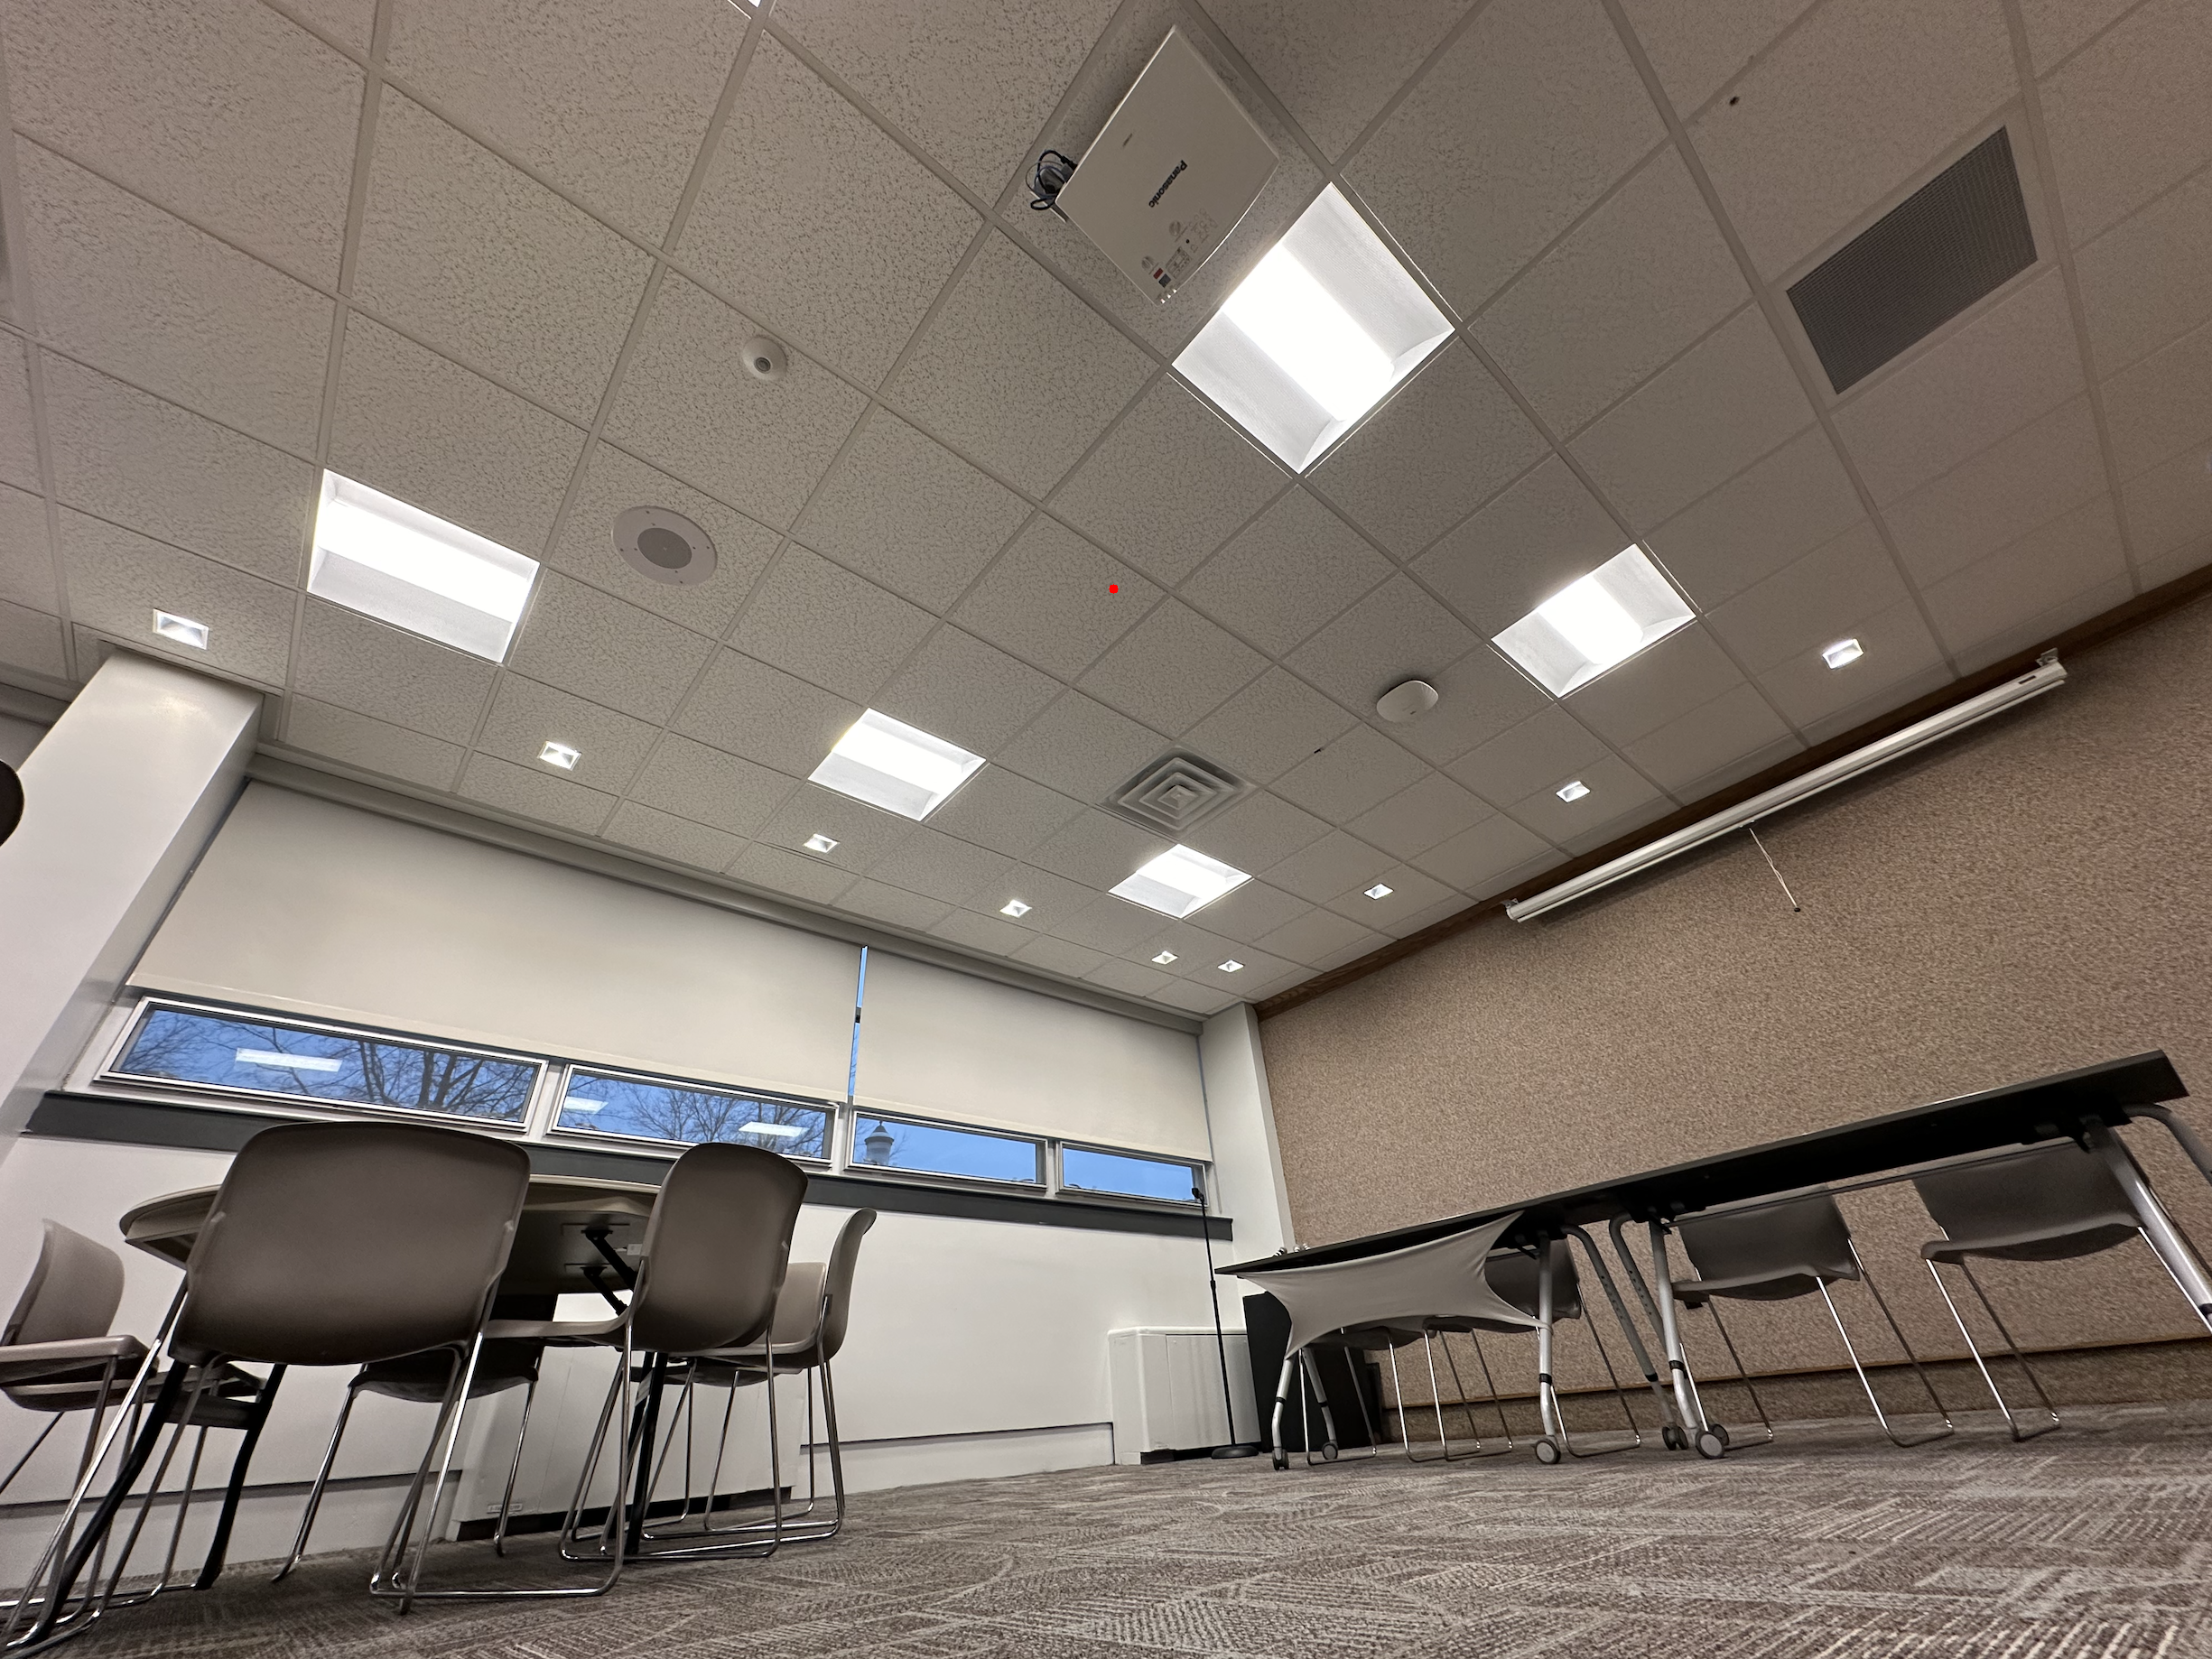
\includegraphics[width=0.8\textwidth]{3vp Centroid of Most Converged Area.png}
    \caption{3VP perspective view Weighted Vanishing Point}
    \label{fig: 3VP perspective view Weighted Vanishing Point}
\end{figure}

\subsection{Person and Pose detection}

\begin{figure}[H]
    \centering
    \includegraphics[width=1.0\textwidth]{1vp person.jpg}
    \caption{Person standing in a 1VP perspective view Scene}
    \label{fig: Person standing in a 1VP perspective view Scene}
\end{figure}

\begin{figure}[H]
    \centering
    \includegraphics[width=1.0\textwidth]{1vp person pose.png}
    \caption{Pose marked person standing in a 1VP perspective view Scene}
    \label{fig: Pose marked person standing in a 1VP perspective view Scene}
\end{figure}


\ref{fig: Person standing in a 1VP perspective view Scene} and \ref{fig: Pose marked person standing in a 1VP perspective view Scene} showcase the a person standing in a 1VP perspective view scene. These images are a part of a video stream that the implementation was tested on. \ref{fig: Pose marked person standing in a 1VP perspective view Scene} Shows the same person with his pose marked over him.\newline

\begin{figure}[H]
    \centering
    \includegraphics[width=1.0\textwidth]{1vp partial person.jpg}
    \caption{Partially visible Person standing in a 1VP perspective view Scene}
    \label{fig: Partially visible Person standing in a 1VP perspective view Scene}
\end{figure}

\ref{fig: Partially visible Person standing in a 1VP perspective view Scene} is from the same video stream as \ref{fig: Person standing in a 1VP perspective view Scene} however here the person is partially occluded behind a desk. \ref{fig: Boundary and pose detected of a partially occluded person} shows the dynamic window created around the person. The person also has a bounding box created around them and their predicted pose marked over them to properly calculate their coordinates.\newline

\begin{figure}[H]
    \centering
    \includegraphics[width=1.0\textwidth]{1vp partial person pose.png}
    \caption{Boundary and pose detected of a partially occluded person}
    \label{fig: Boundary and pose detected of a partially occluded person}
\end{figure}

\subsection{Coordinate calculation and Tracking}

\begin{figure}[H]
    \centering
    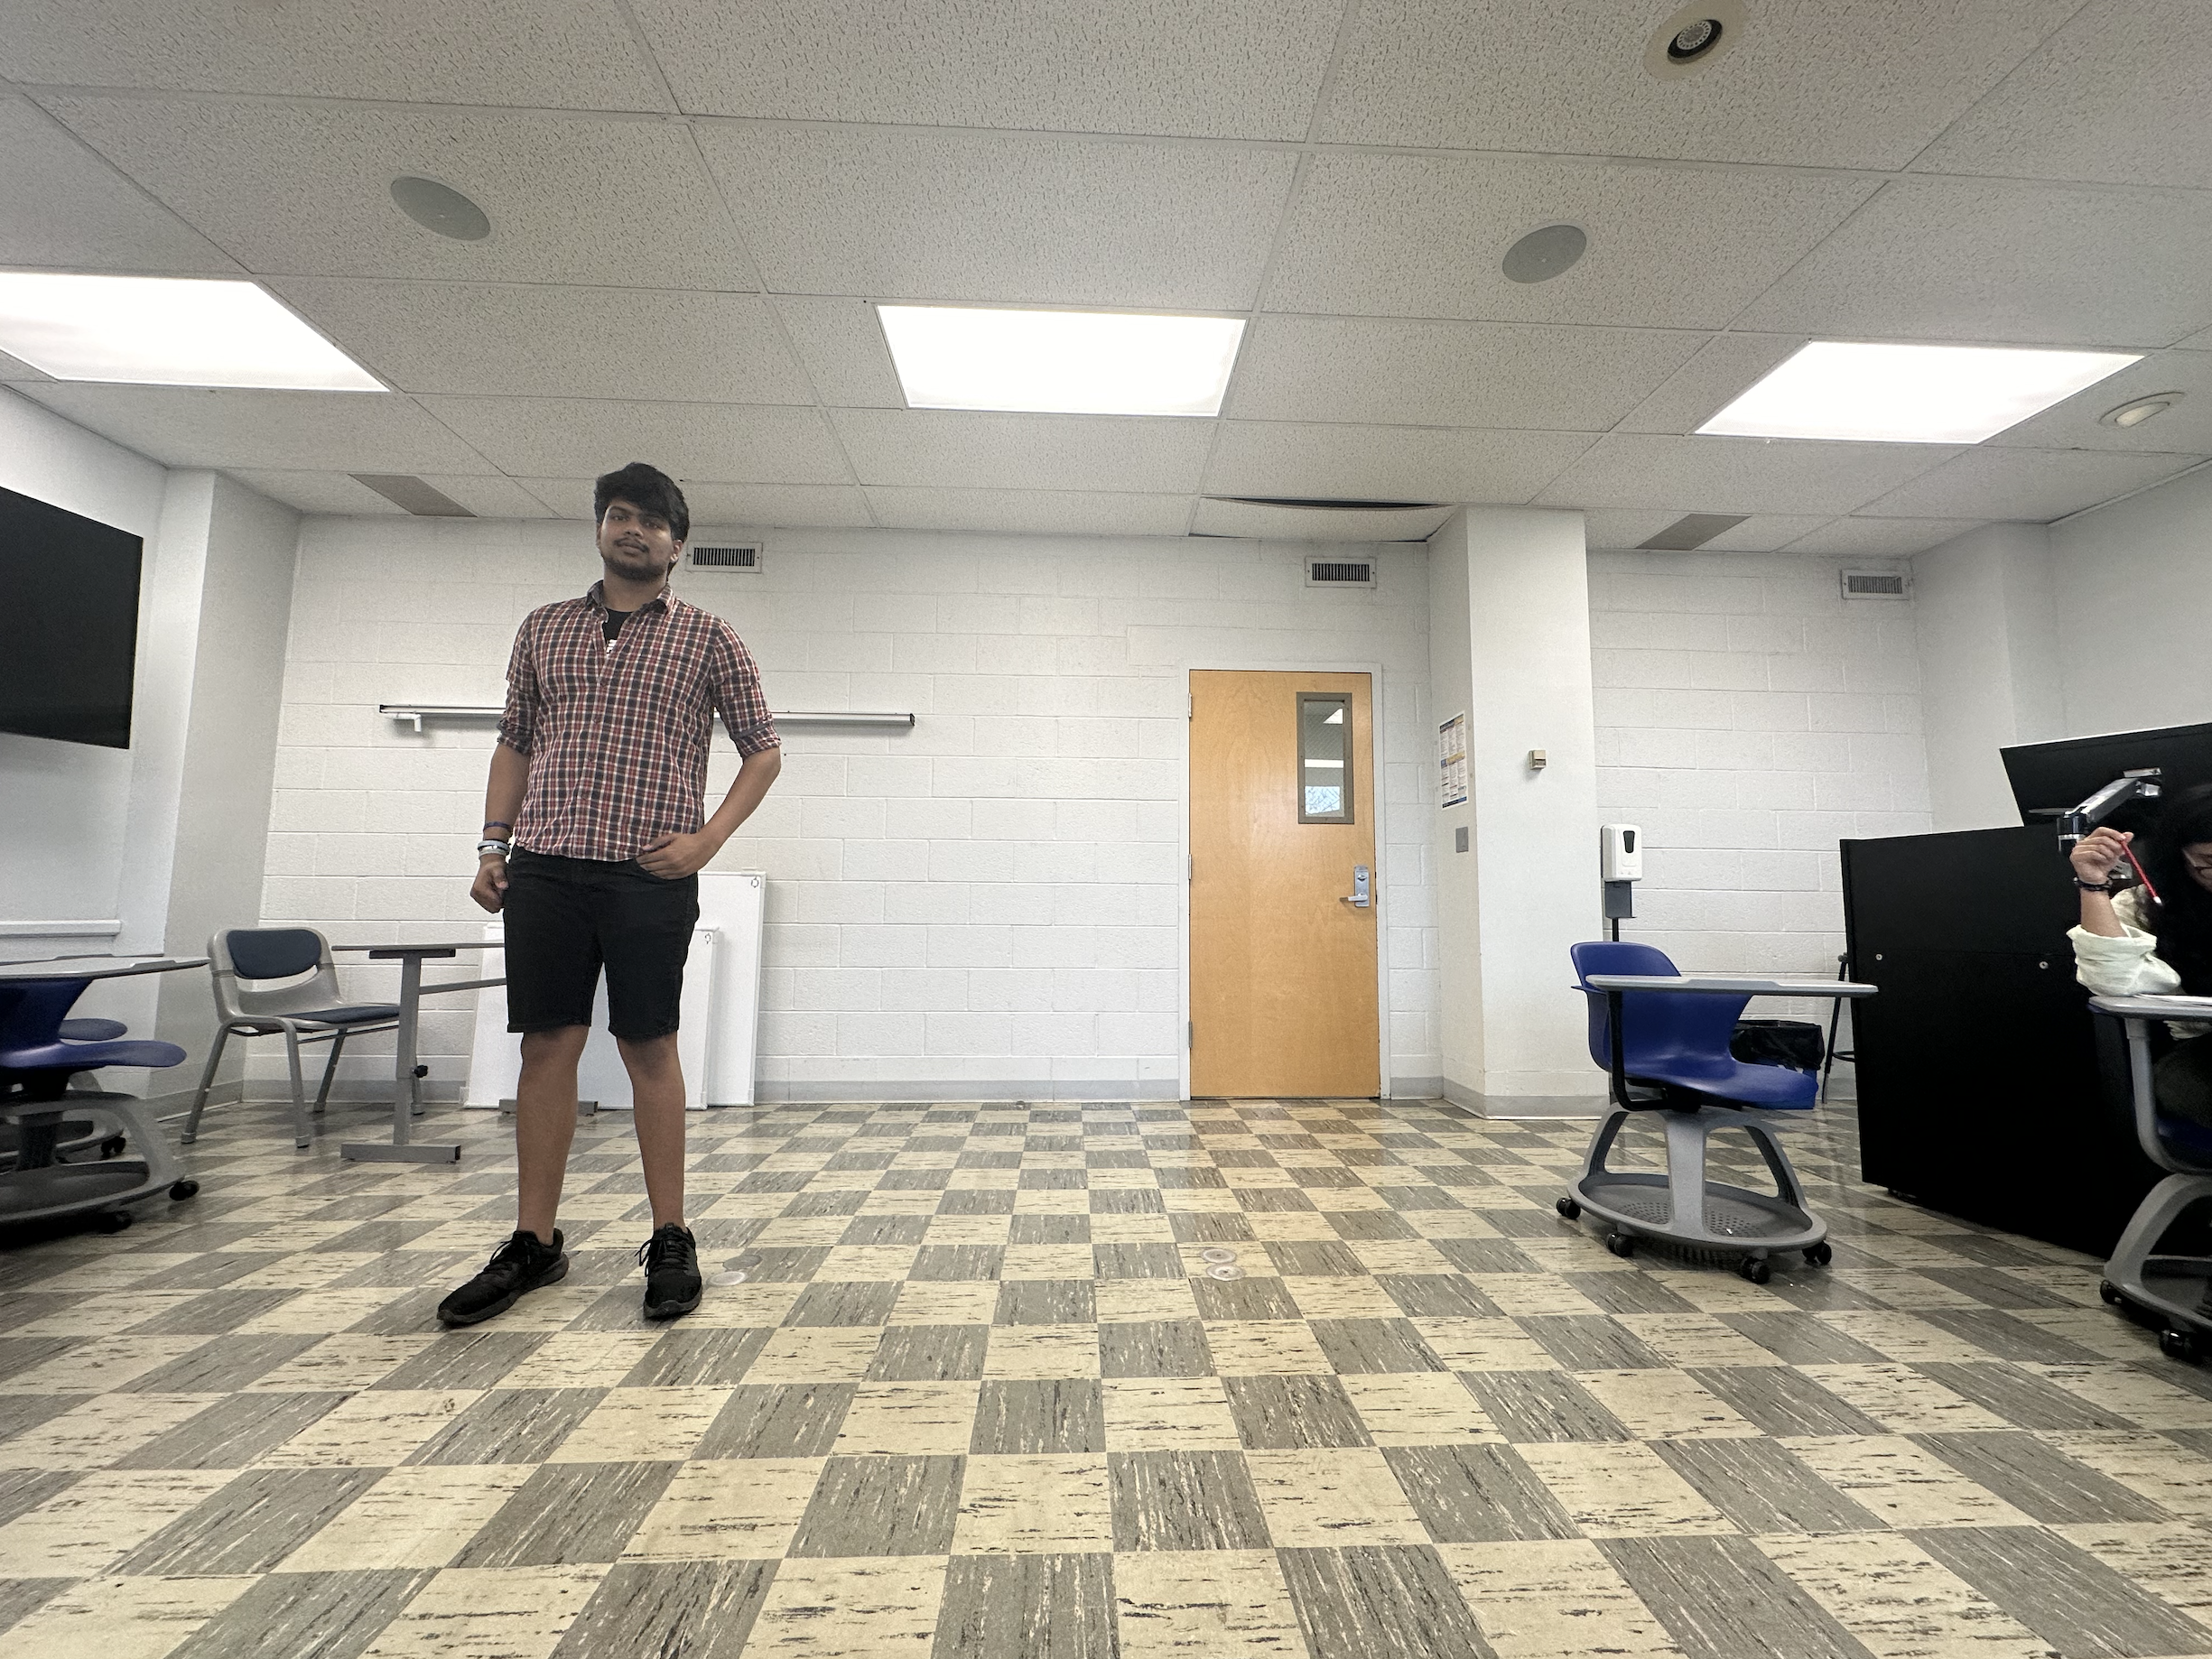
\includegraphics[width=0.8\textwidth]{vineet.png}
    \caption{A tall person in a room}
    \label{fig: A tall person in a room}
\end{figure}

\begin{figure}[H]
    \centering
    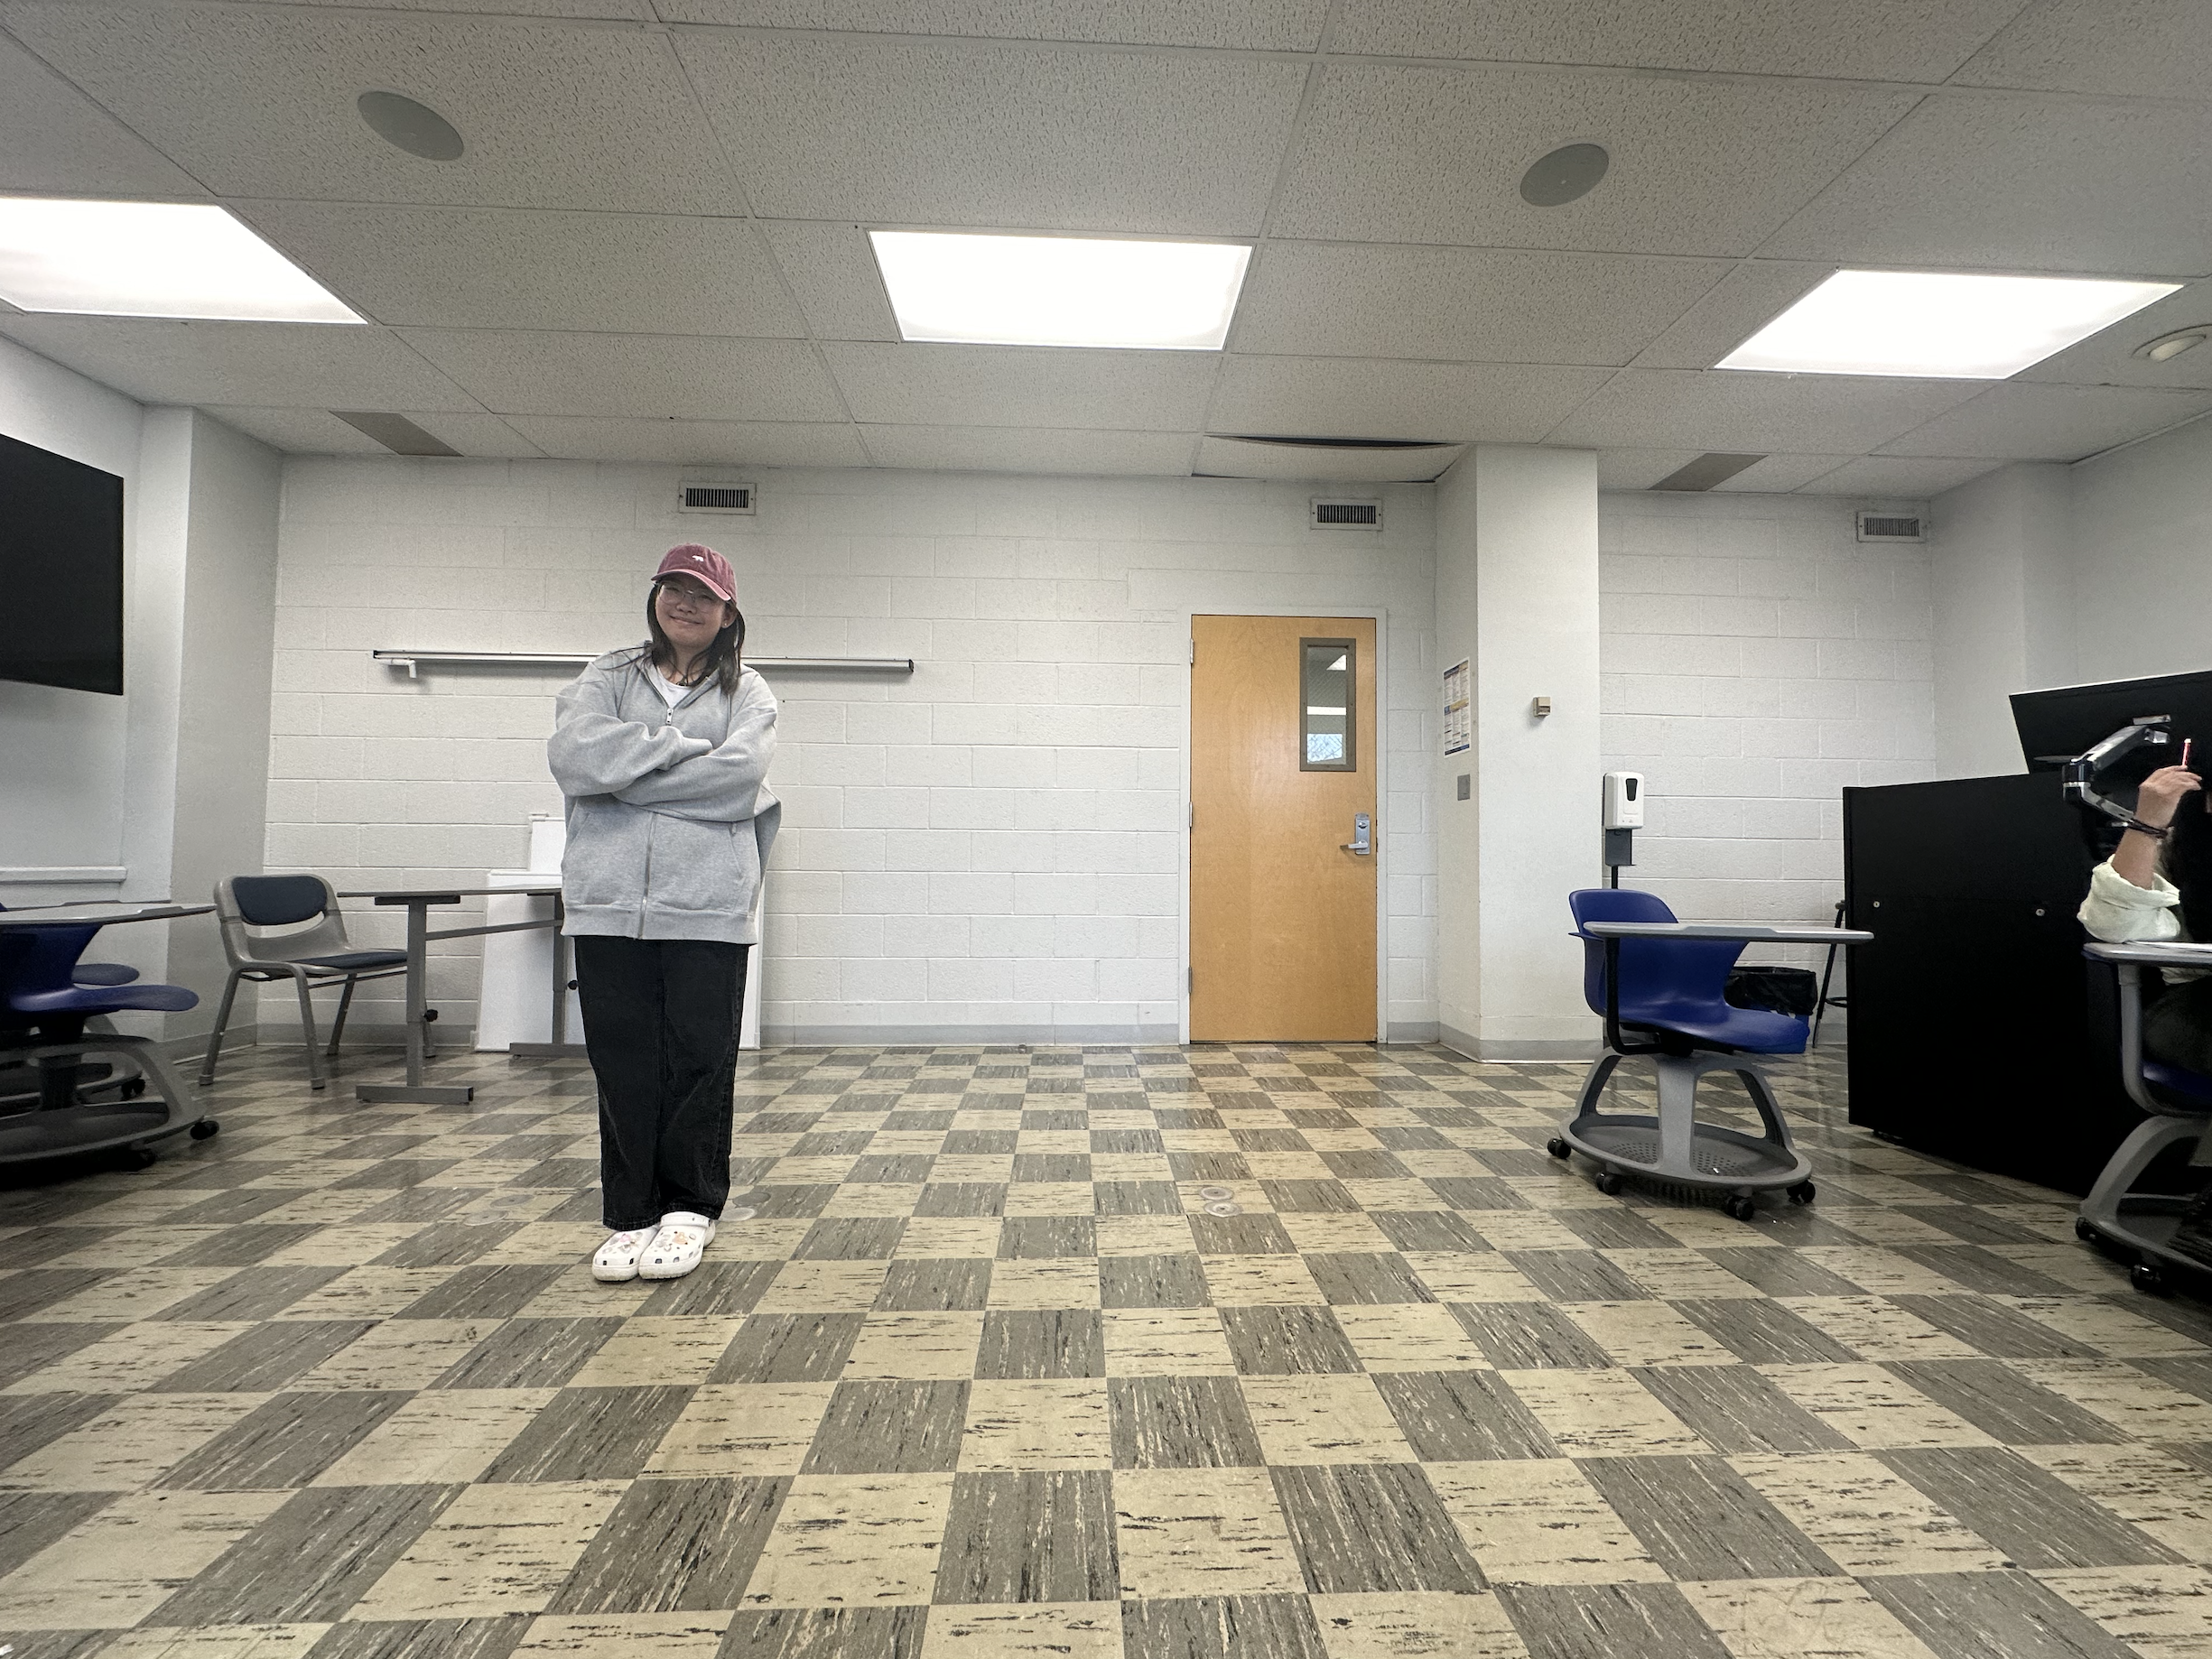
\includegraphics[width=0.8\textwidth]{rexha.png}
    \caption{A short person in a room}
    \label{fig:A short person in a room}
\end{figure}

\begin{figure}[H]
    \centering
    \includegraphics[width=0.8\textwidth]{vineet line.jpeg}
    \caption{Tall person coordinate calculation}
    \label{fig:Tall person coordinate calculation}
\end{figure}

\begin{figure}[H]
    \centering
    \includegraphics[width=0.8\textwidth]{rexha line.jpeg}
    \caption{Short person coordinate calculation}
    \label{fig:Short person coordinate calculation}
\end{figure}

\ref{fig: A tall person in a room} and \ref{fig:A short person in a room} show two people with a significant height difference standing at the same position in the same scene, and \ref{fig:Tall person coordinate calculation} and \ref{fig:Short person coordinate calculation} show the same projection line created for both people. The images and the videos for the testing of the thesis were captured by hand and not a fixed camera with a tripod, therefore there exists a little difference in the field of view of different images and a little camera shake in the videos. These minor imperfections caused by human error present themselves in the form of a reduction of precision and accuracy to a small degree. As long as we can ignore minor errors in the coordinates if they are within an acceptable range, the method yields promising results.\newline
